% SCRUM-102 / A2-T1.2 -- fragment; requires vntex, longtable, array, hyperref.
% Canonical catalog and complete traceability: docs/requirements/srs.md
\section{Yêu cầu chức năng và phi chức năng}
\label{sec:requirements-summary}
\subsection{Cách chuẩn hóa và ưu tiên}

Requirements Specification v3.1 có 46 ID FR và 49 ID NFR. Danh mục SRS hiện hành giữ nguyên ID nguồn; tách FR-CAT-001 thành baseline danh sách và pagination, và FR-PRO-001 thành kiểm tra coupon khi tạo Order và coupon preview. Vì vậy danh mục có 48 dòng FR và 49 dòng NFR, không làm mất yêu cầu nguồn. Mapping UC dựa trên nội dung: UC-PRO-001 xem điểm/ưu đãi; UC-PRO-002 xem trước coupon. Bảng AC, US/UC và vị trí kiểm chứng đầy đủ nằm trong SRS.
\par

MUST và SHOULD biểu thị mức ưu tiên của đặc tả. Ký hiệu MUST* trong bảng nguồn là phân loại đề xuất cho yêu cầu phi chức năng, được giữ để phân biệt với mức ưu tiên tường minh. Các nhóm đặt hàng, thanh toán, idempotency, tồn kho và coupon/loyalty đều được liên kết với tiêu chí kiểm thử.
\par

\subsection{Một số yêu cầu tiêu biểu}
\begingroup\small
\renewcommand{\arraystretch}{1.2}
\begin{longtable}{>{\raggedright\arraybackslash}p{0.10\linewidth}>{\raggedright\arraybackslash}p{0.30\linewidth}>{\raggedright\arraybackslash}p{0.16\linewidth}>{\raggedright\arraybackslash}p{0.34\linewidth}}
\caption{Yêu cầu FR/NFR tiêu biểu}\label{tab:auto-requirements-summary-1}\\
\hline
\textbf{ID} & \textbf{Yêu cầu} & \textbf{Ưu tiên / phạm vi} & \textbf{Tiêu chí và đối chiếu} \\ \hline
\endfirsthead
\textbf{ID} & \textbf{Yêu cầu} & \textbf{Ưu tiên / phạm vi} & \textbf{Tiêu chí và đối chiếu} \\ \hline
\endhead
FR-01 & Guest đăng ký Customer với email chuẩn hóa, email duy nhất và password được hash Argon2id. & MUST; MVP & Dữ liệu hợp lệ tạo đúng một Customer; email trùng không tạo bản ghi thứ hai. V-AUTH; SRS AC-A2-001. \\ \hline
FR-21 & Order chỉ chuyển theo state machine; transition và side effects được xử lý nguyên tử. & MUST; nhất quán giao dịch & Transition ngoài ma trận bị từ chối; trạng thái terminal không bị ghi đè. V-ORDER/V-PAY; SRS AC-A2-021. \\ \hline
FR-27 & Các Order đồng thời không được oversell; thiếu stock phải rollback toàn transaction. & MUST; nhất quán giao dịch & PostgreSQL concurrency test chứng minh không có stock âm hay Order/resource một phần. V-INV; SRS AC-A2-027. \\ \hline
FR-32 & Idempotency-Key ràng buộc theo user; replay cùng payload không lặp payment attempt hoặc side effect. & MUST; nhất quán giao dịch & Kiểm thử replay và key đồng thời trên PostgreSQL; payload khác tuân contract. V-PAY; SRS AC-A2-032. \\ \hline
FR-34 & UI phân biệt pending/unknown, success, failure cuối và kết quả hết hạn; không tin Return URL. & MUST; thanh toán & UI cần nhận trạng thái có thẩm quyền từ backend và phân biệt kết quả cuối với trạng thái đối soát. V-STATUS; SRS AC-A2-034. \\ \hline
FR-38 & QueryDR dùng chung finalization; kết quả không rõ không được suy thành FAILED. & MUST; thanh toán & Kiểm tra state và side effects bằng automated test; kiểm tra tích hợp gateway bằng Sandbox riêng. V-VNP; SRS AC-A2-038. \\ \hline
FR-23 & Hủy chủ động bởi Customer được ghi nhận riêng, không đồng nhất với tự hết hạn Order. & SHOULD; Deferred & Auto-expiration và release tài nguyên vẫn thuộc In Scope; không mặc định có Cancel API/UI. V-ORDER; SRS AC-A2-023. \\ \hline
FR-43 & Coupon preview là yêu cầu riêng với coupon validation lúc tạo Order. & SHOULD; Deferred theo S1/S3/S6 & Đối chiếu request, response, validation và cách xử lý coupon khi tạo đơn. V-PROMO; SRS AC-A2-043. \\ \hline
FR-45 & Loyalty points chỉ cộng đúng một lần khi thanh toán hợp lệ làm Order chuyển PAID. & MUST; thanh toán & Điều kiện theo provider: VNPay trong grace cần payDate đúng hạn và Order chưa CANCELLED; late/ineligible không hồi sinh/cộng điểm; ZERO\_AMOUNT eligible kết thúc với 0 điểm, không gateway/grace; replay không cộng lặp. SRS AC-A2-045. \\ \hline
NFR-01 & JWT được xác minh và ownership được thực thi phía server. & MUST*; bảo mật & Thử hai Customer truy cập chéo bằng integration test; dữ liệu của chủ khác không lộ. V-AUTH/V-ORDER/V-PAY; SRS AC-A2-049. \\ \hline
NFR-03 & Password dùng Argon2id; DB được phép lưu hash/salt, nhưng không persist plaintext hoặc trả/log plaintext/hash. & MUST*; bảo mật & Đối chiếu DB, API response và log capture khi đăng ký/đăng nhập. SRS AC-A2-051. \\ \hline
NFR-10 & Tạo Order, finalization, release, coupon và loyalty phải atomic. & MUST*; nhất quán & Inject lỗi ở từng bước trên PostgreSQL; xác nhận rollback, không có side effect một phần. V-ORDER/V-INV/V-PAY/V-PROMO; SRS AC-A2-058. \\ \hline
NFR-21 & Mục tiêu xử lý nội bộ dưới 500 ms áp dụng trên dữ liệu mẫu/Mock. & MUST; hiệu năng & Đo xử lý server-side trong môi trường/dữ liệu mẫu được ghi rõ; không áp SLA tổng thể cho redirect/IPN/QueryDR bất đồng bộ. V-PAY/V-ORDER; SRS AC-A2-069. \\ \hline
NFR-40 & Môi trường cần tái tạo từ clone sạch theo hướng dẫn Compose và seed. & MUST*; vận hành & Chạy trên DB/volume riêng, ghi cấu hình, health và seed evidence; kiểm tra khả năng tái tạo môi trường. V-OPS; SRS AC-A2-088. \\ \hline
\end{longtable}
\endgroup

\subsection{Cơ sở đặc tả}
Requirements v3.1, User Stories, Use Case Specification và API Contract v4.0 cung cấp cơ sở yêu cầu. Các phiên bản và liên kết nguồn được giữ tại phụ lục\ref{sec:report-provenance} và SRS. Yêu cầu mô tả hành vi mong đợi; hiện thực và kết quả thử nghiệm được trình bày riêng ở các chương sau.

\subsection{Use Case Diagram tổng quát}
SRS §10 liên kết sơ đồ A1 và bản tổng quát cập nhật gồm 14 UC. Guest, Customer, người vận hành demo và VNPay Sandbox là actor ngoài; Mock, ZERO\_AMOUNT và scheduler là nội bộ. UC-ORD-003 chỉ biểu diễn auto-expiration hỗ trợ, không mở Customer Cancel; UC-PRO-002 giữ trạng thái nguồn và acceptance riêng. Không thêm UI Admin/Barista hoặc nghiệp vụ mới.
\par
\noindent\href{https://github.com/brewlite-project/brewlite-a2/blob/6ee4199acaab709471144295adc98ac34e9f11c3/docs/requirements/diagrams/use-case-overview.svg}{Use Case Diagram (SVG)}; \href{https://github.com/brewlite-project/brewlite-a2/blob/6ee4199acaab709471144295adc98ac34e9f11c3/docs/requirements/diagrams/use-case-overview.puml}{Nguồn PlantUML}. Liên kết giữ snapshot nguồn cố định. Hình\ref{fig:use-case-overview} xuất trực tiếp từ danh mục14 UC/4 actor/17 association của PlantUML, chỉ điều chỉnh bố cục để đọc trên A4. Các chú thích phân biệt chức năng tùy chọn và cơ chế nội bộ.
\par
\begin{landscape}
\begin{figure}[p]
\centering
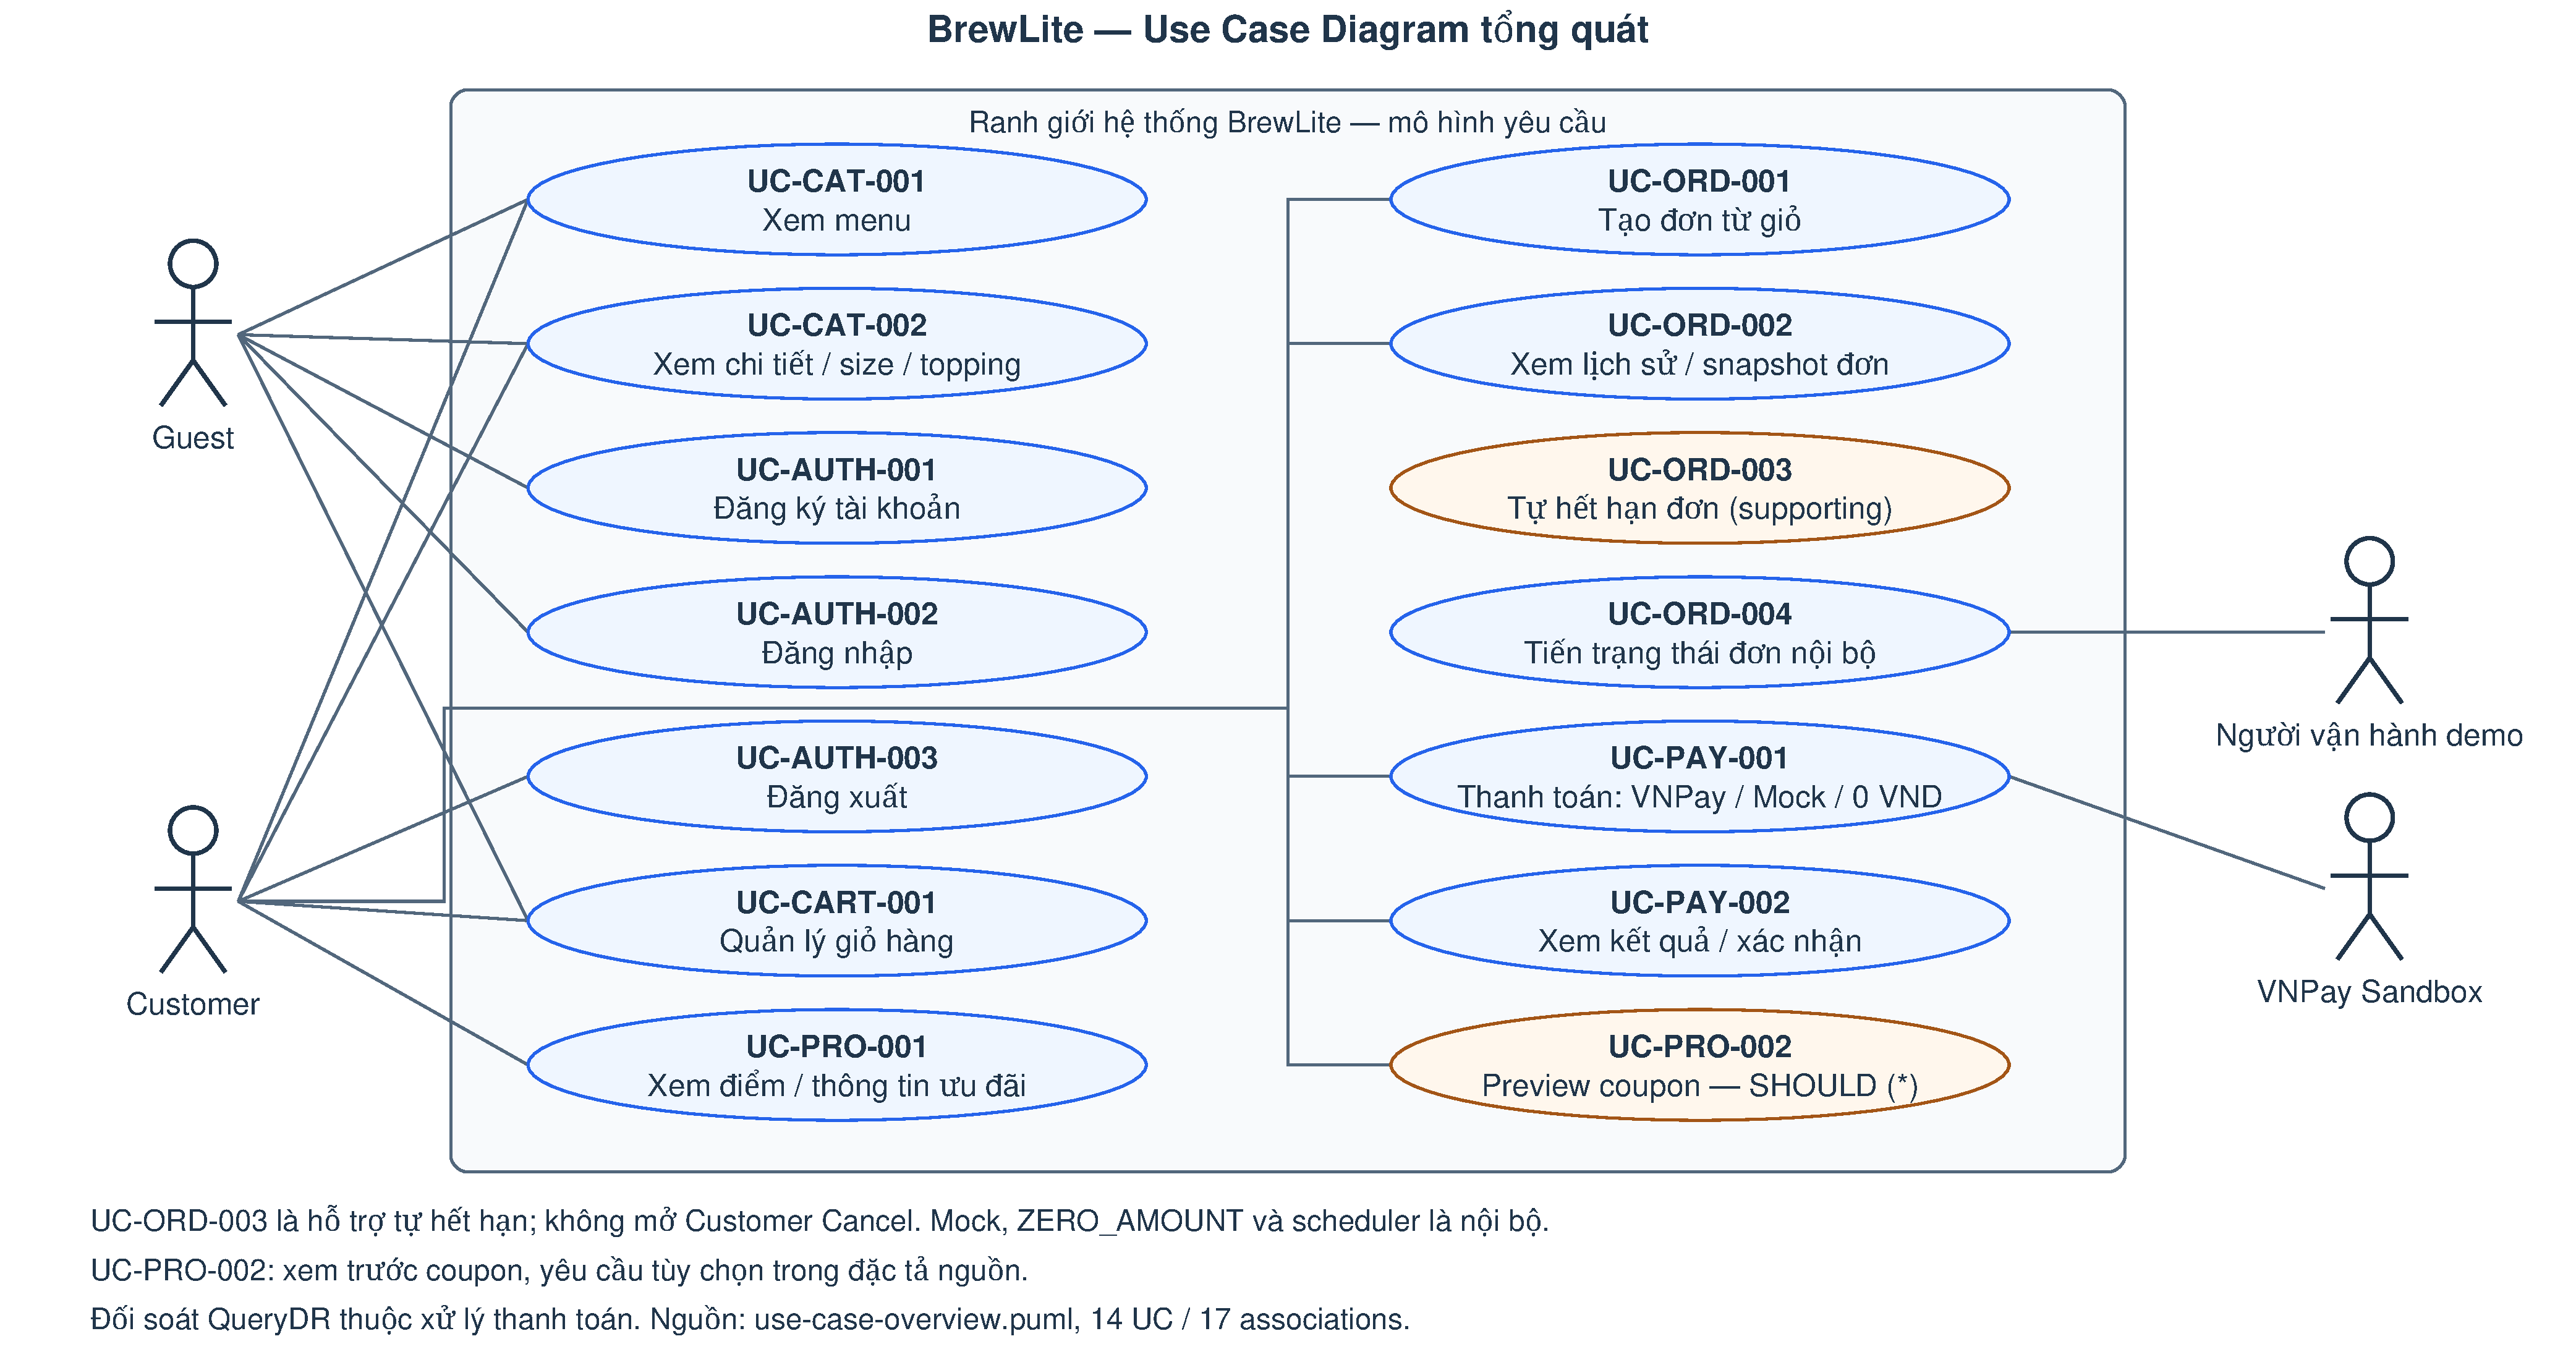
\includegraphics[width=\linewidth,height=0.86\textheight,keepaspectratio]{docs/report/assets/use-case-overview.pdf}
\caption[Use Case Diagram tổng quát của BrewLite]{Use Case Diagram tổng quát: Guest, Customer, người vận hành demo và VNPay Sandbox.
Nguồn chỉnh sửa: \path{docs/requirements/diagrams/use-case-overview.puml};
bản vector dùng cùng actor/UC/quan hệ, không biểu diễn mức hoàn thành chức năng.}
\label{fig:use-case-overview}
\end{figure}
\end{landscape}

\subsection{Yêu cầu tích hợp liên tục}
NFR-38 yêu cầu pipeline tự động cài dependency theo lockfile, lint, unit test và build cho cả web/API khi cập nhật pull request. Kết quả được gắn với source tương ứng; CI ứng dụng không thay kiểm thử tích hợp database hoặc giao dịch Sandbox.
\par

\subsection{Yêu cầu vận hành và triển khai}
Các yêu cầu vận hành bao gồm giao diện mobile-first, HTTPS, CI/CD, khả năng theo dõi tình trạng dịch vụ và phục hồi khi triển khai gặp lỗi. Bảng dưới hệ thống hóa tiêu chí theo đề học phần; đây là đặc tả, không phải bảng kết quả thực nghiệm.
\par
\begingroup\small
\renewcommand{\arraystretch}{1.2}
\begin{longtable}{>{\raggedright\arraybackslash}p{0.17\linewidth}>{\raggedright\arraybackslash}p{0.25\linewidth}>{\raggedright\arraybackslash}p{0.44\linewidth}}
\caption{Yêu cầu vận hành và tiêu chí}\label{tab:auto-requirements-summary-2}\\
\hline
\textbf{ID / ưu tiên} & \textbf{Task / liên kết} & \textbf{Tiêu chí tiêu biểu} \\ \hline
\endfirsthead
\textbf{ID / ưu tiên} & \textbf{Task / liên kết} & \textbf{Tiêu chí tiêu biểu} \\ \hline
\endhead
A2-OPS-01 / MUST: PWA / mobile-first & Task 3 kiến trúc; Task 4 giao diện; Task 5 kiểm chứng; NFR-25, NFR-28; S11 Task 3/5 & AC-OPS-01: Given web chạy trên trình duyệt/viewport mục tiêu được ghi rõ, When kiểm tra manifest, icons, installability và UI, Then có bằng chứng PWA theo khả năng hỗ trợ của trình duyệt; ghi giới hạn hỗ trợ. Không tự yêu cầu offline checkout, sync hay native app. \\ \hline
A2-OPS-02 / MUST: HTTPS và ranh giới triển khai & Task 3 deployment/ADR; Task 5 production; NFR-04/43/44/49; S11 Task 3/5 & AC-OPS-02: Given URLs public của web/API, When truy cập từ ngoài môi trường local, Then HTTPS/certificate hợp lệ, không mixed content; DB không public; secrets chỉ backend. Lưu URLs và kết quả kiểm tra không chứa secret. \\ \hline
A2-OPS-03 / MUST: CI bắt buộc & Task 4.4; NFR-38 / AC-A2-086; REQ-02 PR \#7; S11 Task 4 & AC-OPS-03: Thực hiện toàn bộ AC-A2-086: Install  $\rightarrow$  Lint  $\rightarrow$  Unit Test  $\rightarrow$  Build; required checks chặn merge, evidence PR xanh/đỏ trên đúng commit. \\ \hline
A2-OPS-04 / MUST: CD và release & Task 3 ADR; Task 5 CD/deploy; NFR-32/40/41/42/49; S11 Task 5 & AC-OPS-04: Given release đã qua quality gates, When CD thực thi, Then deploy đúng artifact/image có version truy vết tới commit, cấu hình secrets an toàn và migration có kiểm soát; lỗi gate/migration/deploy làm dừng luồng hoặc xử lý theo rollback đã định. Lưu workflow/run URL, version và deploy evidence. \\ \hline
A2-OPS-05 / MUST: Health và DB readiness & Task 3 thiết kế; Task 5 implementation/verification; NFR-16/40/49; S11 Task 5 & AC-OPS-05: Given hệ thống chạy, When kiểm tra health và trạng thái DB, Then xác định được khả năng phục vụ và DB readiness theo cơ chế được task thiết kế chốt; thử DB mất kết nối cho kết quả degraded/not-ready phù hợp. Không coi GET / liveness hiện có là bằng chứng DB-ready; không tự định nghĩa route mới tại đây. \\ \hline
A2-OPS-06 / MUST: Production smoke test & Task 5 QA/deployment; FR-08/19/22/30/34; NFR-25/33/40; S11 Task 5 & AC-OPS-06: Given version vừa deploy, When chạy smoke trên web/API HTTPS và luồng menu  $\rightarrow$  auth  $\rightarrow$  tạo đơn  $\rightarrow$  payment demo được cho phép  $\rightarrow$  xác nhận/lịch sử, Then các bước đạt expected result theo contract. Ghi version, URLs, thời điểm, môi trường và kết quả từng bước; lỗi làm dừng release hoặc kích hoạt xử lý đã định. Không dùng tiền thật, không bật Mock production trái policy, không dùng synthetic làm Sandbox E2E. \\ \hline
A2-OPS-07 / MUST: Rollback và runbook & Task 3 chiến lược; Task 5 release/rollback; NFR-10/16/32/40/41; S11 Task 5 & AC-OPS-07: Given release lỗi, When thực hiện runbook rollback đã duyệt, Then có thể quay về artifact/version trước tương thích dữ liệu và xác minh lại health/smoke; ghi trigger, người thực hiện, version và kết quả. Migration có giới hạn/chiến lược tương thích rõ, không giả định có thể đảo DB phá hủy tự động. \\ \hline
\end{longtable}
\endgroup
Quy trình kiểm chứng cần ghi rõ môi trường, dữ liệu mẫu, phiên bản và kết quả quan sát để có thể tái lập.
\par


\subsection{User stories và tiêu chí kiểm chứng toàn luồng}
SRS kế thừa14 UC,43 stories Phase1 và49 stories tổng cộng khi có6 US-VNP;
253 AC của nguồn stories không đồng nhất với97 dòng FR/NFR hoặc8 AC delivery.
Theo góc nhìn Customer, US-CAT/US-CART nối menu--tùy chọn--giỏ; US-ORD nối tạo
đơn/lịch sử; US-PAY/US-VNP nối thanh toán/trạng thái; US-PRO nối coupon/điểm.
Tên/ID chi tiết giữ catalog nguồn, không tạo story mới cho NFR.

Một tiêu chí có thể kiểm chứng phải ghi input, expected outcome và môi trường:
ví dụ FR-27 cần request cạnh tranh trên PostgreSQL chứng minh không oversell;
FR-32 cần replay cùng key/payload không lặp side effect; FR-34 cần UI phân
biệt unknown và terminal outcome theo server. Response thành công một lần
không thay các case lỗi, ownership hoặc duplicate. Mapping cụ thể US/UC và
test inventory nằm ở matrix; kết quả thực nghiệm được trình bày ở chương kiểm thử.
